\documentclass[twocolumn]{article}
\usepackage[utf8]{inputenc}
\usepackage[T1]{fontenc}
\usepackage{amsmath,amssymb,amsfonts}
\usepackage{graphicx}
\usepackage{booktabs}
\usepackage{hyperref}
\usepackage[margin=0.85in]{geometry}
\usepackage{caption}
\usepackage{subcaption}
\usepackage{float}
\usepackage{authblk}
\usepackage{times}
\usepackage{microtype}
\usepackage{xcolor}

\title{Synthetic Data Augmentation for Breast Ultrasound Lesion Segmentation via Generative Flow Matching}

\author[1]{Ali Rouzbayani}
\author[3]{Zlatitsa Todorova}
\author[3]{Dev Patel}
\author[3,4]{Errol Camlioglu}
\author[1]{Rayan Sadri}

\affil[1]{AI Research, Carez Inc., Austin, TX, USA}
\affil[3]{Faculty of Medicine and Health Sciences, McGill University, Montreal, QC, Canada}
\affil[4]{Department of Radiology, Jewish General Hospital, Montreal, QC, Canada}

\date{}

\begin{document}
\maketitle

% ============================================================
\begin{abstract}
Training accurate segmentation models for breast ultrasound imaging is hindered by the scarcity of annotated data and the high cost of expert labeling. In this work, we propose a pipeline for generating synthetic ultrasound image--mask pairs using an unconditional UNet-based generative model (106.4M parameters) trained with a flow matching objective, and evaluate the downstream impact of synthetic data augmentation on lesion segmentation performance. We train the generative model on 556 annotated breast ultrasound images and produce up to 1{,}000 synthetic image--mask pairs. A systematic experiment augmenting the real training set with varying quantities of synthetic samples---repeated across three random seeds---reveals that synthetic augmentation consistently improves segmentation: adding 1{,}000 synthetic samples yields a Dice score of $0.823 \pm 0.004$ compared to a baseline of $0.797 \pm 0.014$, a relative improvement of 3.3\%. A t-SNE analysis confirms strong distributional overlap between real and synthetic samples. These findings demonstrate the potential of flow matching generative models to address data scarcity in medical image segmentation.

\medskip
\noindent\textbf{Keywords:} Synthetic Data, Flow Matching, Diffusion Models, Breast Ultrasound, Lesion Segmentation, UNet, Medical Imaging
\end{abstract}

% ============================================================
\section{Introduction}
\label{sec:intro}

Artificial intelligence has been increasingly adopted in diagnostic and interventional radiology, enabling the automated detection, segmentation, and visualization of pathological lesions and anatomical structures across imaging modalities~\cite{litjens2017}. Segmentation models, in particular, play a central role in assisting clinicians during diagnostic workflows and real-time interventional procedures. However, training such models requires large volumes of annotated imaging data---a resource that is expensive, logistically complex, and ethically constrained to obtain.

Medical imaging datasets are inherently small and sparse: with only a few hundred annotated samples, a segmentation model observes a narrow slice of the true variability in lesion shape, size, texture, and anatomical context. Traditional data augmentation---geometric transforms, intensity jitter---helps but is fundamentally limited to rearrangements of existing samples; it cannot populate unexplored regions of the data manifold with genuinely novel examples. Acquiring additional real data is costly and logistically complex, requiring collaboration with clinical sites, institutional review board approvals, and expert annotators, with per-dataset costs reaching thousands of dollars~\cite{willemink2020}. Class imbalance further compounds the problem: rare pathologies are underrepresented in training sets, leading to models that underperform on clinically critical cases~\cite{johnson2019}. Generative models offer a fundamentally different approach---by learning the underlying data distribution, they can synthesize novel samples that densify the sparse training manifold, effectively expanding dataset coverage without additional patient data collection.

Synthetic data generation has emerged as a promising approach to alleviate these challenges. Generative models---including Generative Adversarial Networks (GANs)~\cite{goodfellow2014}, Variational Autoencoders (VAEs)~\cite{kingma2014}, and Diffusion Models~\cite{ho2020}---can produce realistic medical images from learned data distributions, enabling dataset expansion without additional patient data collection. Among these, diffusion-based approaches have recently demonstrated state-of-the-art image quality with strong mode coverage~\cite{dhariwal2021}, making them particularly well-suited for medical imaging applications where diversity and fidelity are paramount.

In this work, we adopt a \emph{flow matching} formulation~\cite{lipman2023}, a continuous-time generative framework that offers training stability and simplicity over traditional diffusion models. We train an unconditional UNet-based generative model to jointly produce breast ultrasound images and their corresponding binary segmentation masks as two-channel outputs. We then conduct a systematic study of synthetic data augmentation for downstream lesion segmentation, evaluating the effect of varying synthetic-to-real data ratios on held-out test performance.

Our contributions are as follows:
\begin{enumerate}
    \item We present a complete pipeline for generating paired synthetic ultrasound images and segmentation masks using UNet-based flow matching.
    \item We conduct a controlled, multi-seed experiment demonstrating that synthetic augmentation consistently improves segmentation performance across all augmentation ratios tested.
    \item We provide distributional analysis via t-SNE confirming that generated samples faithfully cover the real data manifold.
\end{enumerate}

% ============================================================
\section{Background}
\label{sec:background}

\subsection{Diffusion Models}

Diffusion models~\cite{ho2020,sohl2015} define a generative process by learning to reverse a gradual noising procedure. In the forward process, Gaussian noise is incrementally added to data $\mathbf{x}_0 \sim p_{\text{data}}$ over $T$ timesteps:
\begin{equation}
    q(\mathbf{x}_t \mid \mathbf{x}_{t-1}) = \mathcal{N}\!\left(\mathbf{x}_t;\, \sqrt{1 - \beta_t}\, \mathbf{x}_{t-1},\, \beta_t \mathbf{I}\right),
\end{equation}
where $\{\beta_t\}_{t=1}^{T}$ is a variance schedule. The reverse process, parameterized by a neural network $\epsilon_\theta$, learns to denoise samples:
\begin{equation}
    p_\theta(\mathbf{x}_{t-1} \mid \mathbf{x}_t) = \mathcal{N}\!\left(\mathbf{x}_{t-1};\, \boldsymbol{\mu}_\theta(\mathbf{x}_t, t),\, \sigma_t^2 \mathbf{I}\right).
\end{equation}
Training minimizes the mean squared error between predicted and actual noise:
\begin{equation}
    \mathcal{L}_{\text{DDPM}} = \mathbb{E}_{t, \mathbf{x}_0, \boldsymbol{\epsilon}}\!\left[\left\|\boldsymbol{\epsilon} - \boldsymbol{\epsilon}_\theta(\mathbf{x}_t, t)\right\|^2\right].
\end{equation}

While effective, the discrete-time formulation requires many denoising steps at inference and can be sensitive to the noise schedule. These limitations motivate continuous-time alternatives.

\subsection{Flow Matching}

Flow matching~\cite{lipman2023,liu2023} recasts generative modeling as learning a time-dependent velocity field that transports samples from a noise distribution to the data distribution along straight paths. Given data $\mathbf{x}_1 \sim p_{\text{data}}$ and noise $\mathbf{x}_0 \sim \mathcal{N}(\mathbf{0}, \mathbf{I})$, the interpolation path is defined as:
\begin{equation}
    \mathbf{x}_t = (1 - t)\,\mathbf{x}_0 + t\,\mathbf{x}_1, \quad t \in [0, 1].
    \label{eq:interpolation}
\end{equation}
The target velocity field is the time derivative of this path:
\begin{equation}
    \mathbf{v}^*(\mathbf{x}_t, t) = \frac{d\mathbf{x}_t}{dt} = \mathbf{x}_1 - \mathbf{x}_0.
    \label{eq:velocity}
\end{equation}
A neural network $\mathbf{v}_\theta$ is trained to regress this velocity:
\begin{equation}
    \mathcal{L}_{\text{FM}} = \mathbb{E}_{t \sim \mathcal{U}(0,1),\, \mathbf{x}_0,\, \mathbf{x}_1}\!\left[\left\|\mathbf{v}_\theta(\mathbf{x}_t, t) - (\mathbf{x}_1 - \mathbf{x}_0)\right\|^2\right].
    \label{eq:fm_loss}
\end{equation}
At inference, new samples are generated by solving the ordinary differential equation (ODE):
\begin{equation}
    \frac{d\mathbf{x}_t}{dt} = \mathbf{v}_\theta(\mathbf{x}_t, t), \quad \mathbf{x}_0 \sim \mathcal{N}(\mathbf{0}, \mathbf{I}),
    \label{eq:ode}
\end{equation}
from $t = 0$ to $t = 1$ using a numerical solver (e.g., Euler method). Compared to DDPM, flow matching offers several advantages: (1) a simpler training objective without noise schedule tuning, (2) straight interpolation paths that require fewer solver steps, and (3) stable training dynamics~\cite{lipman2023}.

\subsection{UNet vs.\ Transformer-Based Architectures}

Two dominant backbone architectures have been employed for diffusion and flow matching models: UNet~\cite{ronneberger2015} and Diffusion Transformers (DiT)~\cite{peebles2023}. DiT leverages self-attention to capture long-range dependencies and has achieved state-of-the-art results on large-scale benchmarks~\cite{peebles2023}. However, its scalability advantages depend on large training sets; transformers are data-hungry and lack the built-in spatial priors that convolutional networks provide. The UNet architecture, with its encoder--decoder structure, skip connections, and multi-scale convolutional feature extraction, encodes a strong inductive bias toward spatial locality and translation equivariance. These properties make UNet well-suited for pixel-level generation tasks on small datasets, where the model must produce spatially coherent outputs without the benefit of millions of training examples. For this reason, we adopt a UNet backbone in this work.

% ============================================================
\section{Methods}
\label{sec:methods}

\subsection{Dataset}

We use the publicly available Breast Ultrasound Images (BUSI) dataset~\cite{al-dhabyani2020}, which contains 780 grayscale ultrasound images across three classes: benign (437), malignant (210), and normal (133). We exclude the 133 normal images (which contain no lesions) and use the remaining 647 images with corresponding binary lesion segmentation masks. Some images contain multiple annotated masks for distinct lesion regions; we aggregate these into a single binary mask per image via logical OR. All images are resized to $128 \times 128$ pixels.

The dataset is randomly split into training (556 images, 86\%), validation (45 images, 7\%), and test (46 images, 7\%) sets with a fixed random seed.

\subsection{Generative Model}

We train an unconditional generative model to produce paired ultrasound images and segmentation masks simultaneously. Each training sample is represented as a two-channel tensor $\mathbf{x} \in \mathbb{R}^{2 \times 128 \times 128}$, where channel 0 contains the grayscale image normalized to $[-1, 1]$ and channel 1 contains the binary mask similarly normalized.

The velocity field $\mathbf{v}_\theta$ is parameterized by a \texttt{UNet2DModel} from the Diffusers library~\cite{von-platen2022} with 2 input and 2 output channels, block channels $(128, 256, 512, 512)$, attention at the two deepest scales, and 2 layers per block, totaling 106.4M parameters. The model is conditioned on the continuous timestep $t$ via sinusoidal positional embeddings.

Training follows the flow matching objective (Eq.~\ref{eq:fm_loss}) with the AdamW optimizer ($\text{lr} = 10^{-4}$, weight decay $= 10^{-4}$), cosine annealing learning rate schedule, gradient clipping at norm 1.0, and batch size 8. The model is trained for 300 epochs on a single NVIDIA A100-80GB GPU, converging to a best validation loss of 0.055.

At inference, we generate samples using an Euler ODE solver with 100 steps. The image channel is directly output, while the mask channel is binarized at a threshold of 0.5.

\subsection{Segmentation Model}

For downstream evaluation, we train a standard UNet segmentation model~\cite{ronneberger2015} with an encoder--decoder architecture (channel widths 32--64--128--256--512) and skip connections, totaling 7.8M parameters.

The model is trained with a combined Dice + binary cross-entropy loss:
\begin{equation}
    \mathcal{L}_{\text{seg}} = \mathcal{L}_{\text{BCE}} + \left(1 - \frac{2\sum_i p_i g_i + 1}{\sum_i p_i + \sum_i g_i + 1}\right),
\end{equation}
where $p_i$ and $g_i$ are the predicted and ground-truth values at pixel $i$. We use the AdamW optimizer ($\text{lr} = 10^{-3}$, weight decay $= 10^{-4}$), cosine annealing, and train for 200 epochs with batch size 16.

\textbf{Data augmentation.} Both baseline and synthetic-augmented experiments apply identical augmentations: random horizontal/vertical flips, rotation ($\pm 15°$), affine transformations (scale 0.85--1.15, translation $\pm 10$ pixels), brightness and contrast jitter (factor 0.8--1.2), and Gaussian blur (radius 0.5--1.5). This ensures that any performance differences are attributable solely to the addition of synthetic data.

\subsection{Experimental Design}

We conduct a controlled experiment to evaluate the impact of synthetic data augmentation on segmentation performance:

\begin{enumerate}
    \item \textbf{Baseline:} Segmentation model trained on 556 real images with standard augmentation.
    \item \textbf{Synthetic-augmented:} Same model trained on 556 real images plus $N$ synthetic image--mask pairs ($N \in \{100, 200, \ldots, 1000\}$) with identical augmentation.
\end{enumerate}

All experiments are evaluated on the same held-out test set (46 images) using four metrics: Dice coefficient, Intersection over Union (IoU), precision, and recall. To account for training stochasticity, each configuration is repeated across three random seeds and results are reported as mean $\pm$ standard deviation.

% ============================================================
\section{Results}
\label{sec:results}

\subsection{Quality of Generated Samples}

Figure~\ref{fig:real_vs_gen} presents a side-by-side comparison of real and generated samples. The real images and masks (rows 1--2) are drawn from the held-out test set, while the generated pairs (rows 3--4) are produced by the flow matching model. The synthetic images exhibit realistic speckle texture, tissue boundaries, and lesion morphology, with spatially coherent masks that align with hypoechoic regions.

\begin{figure}[t]
    \centering
    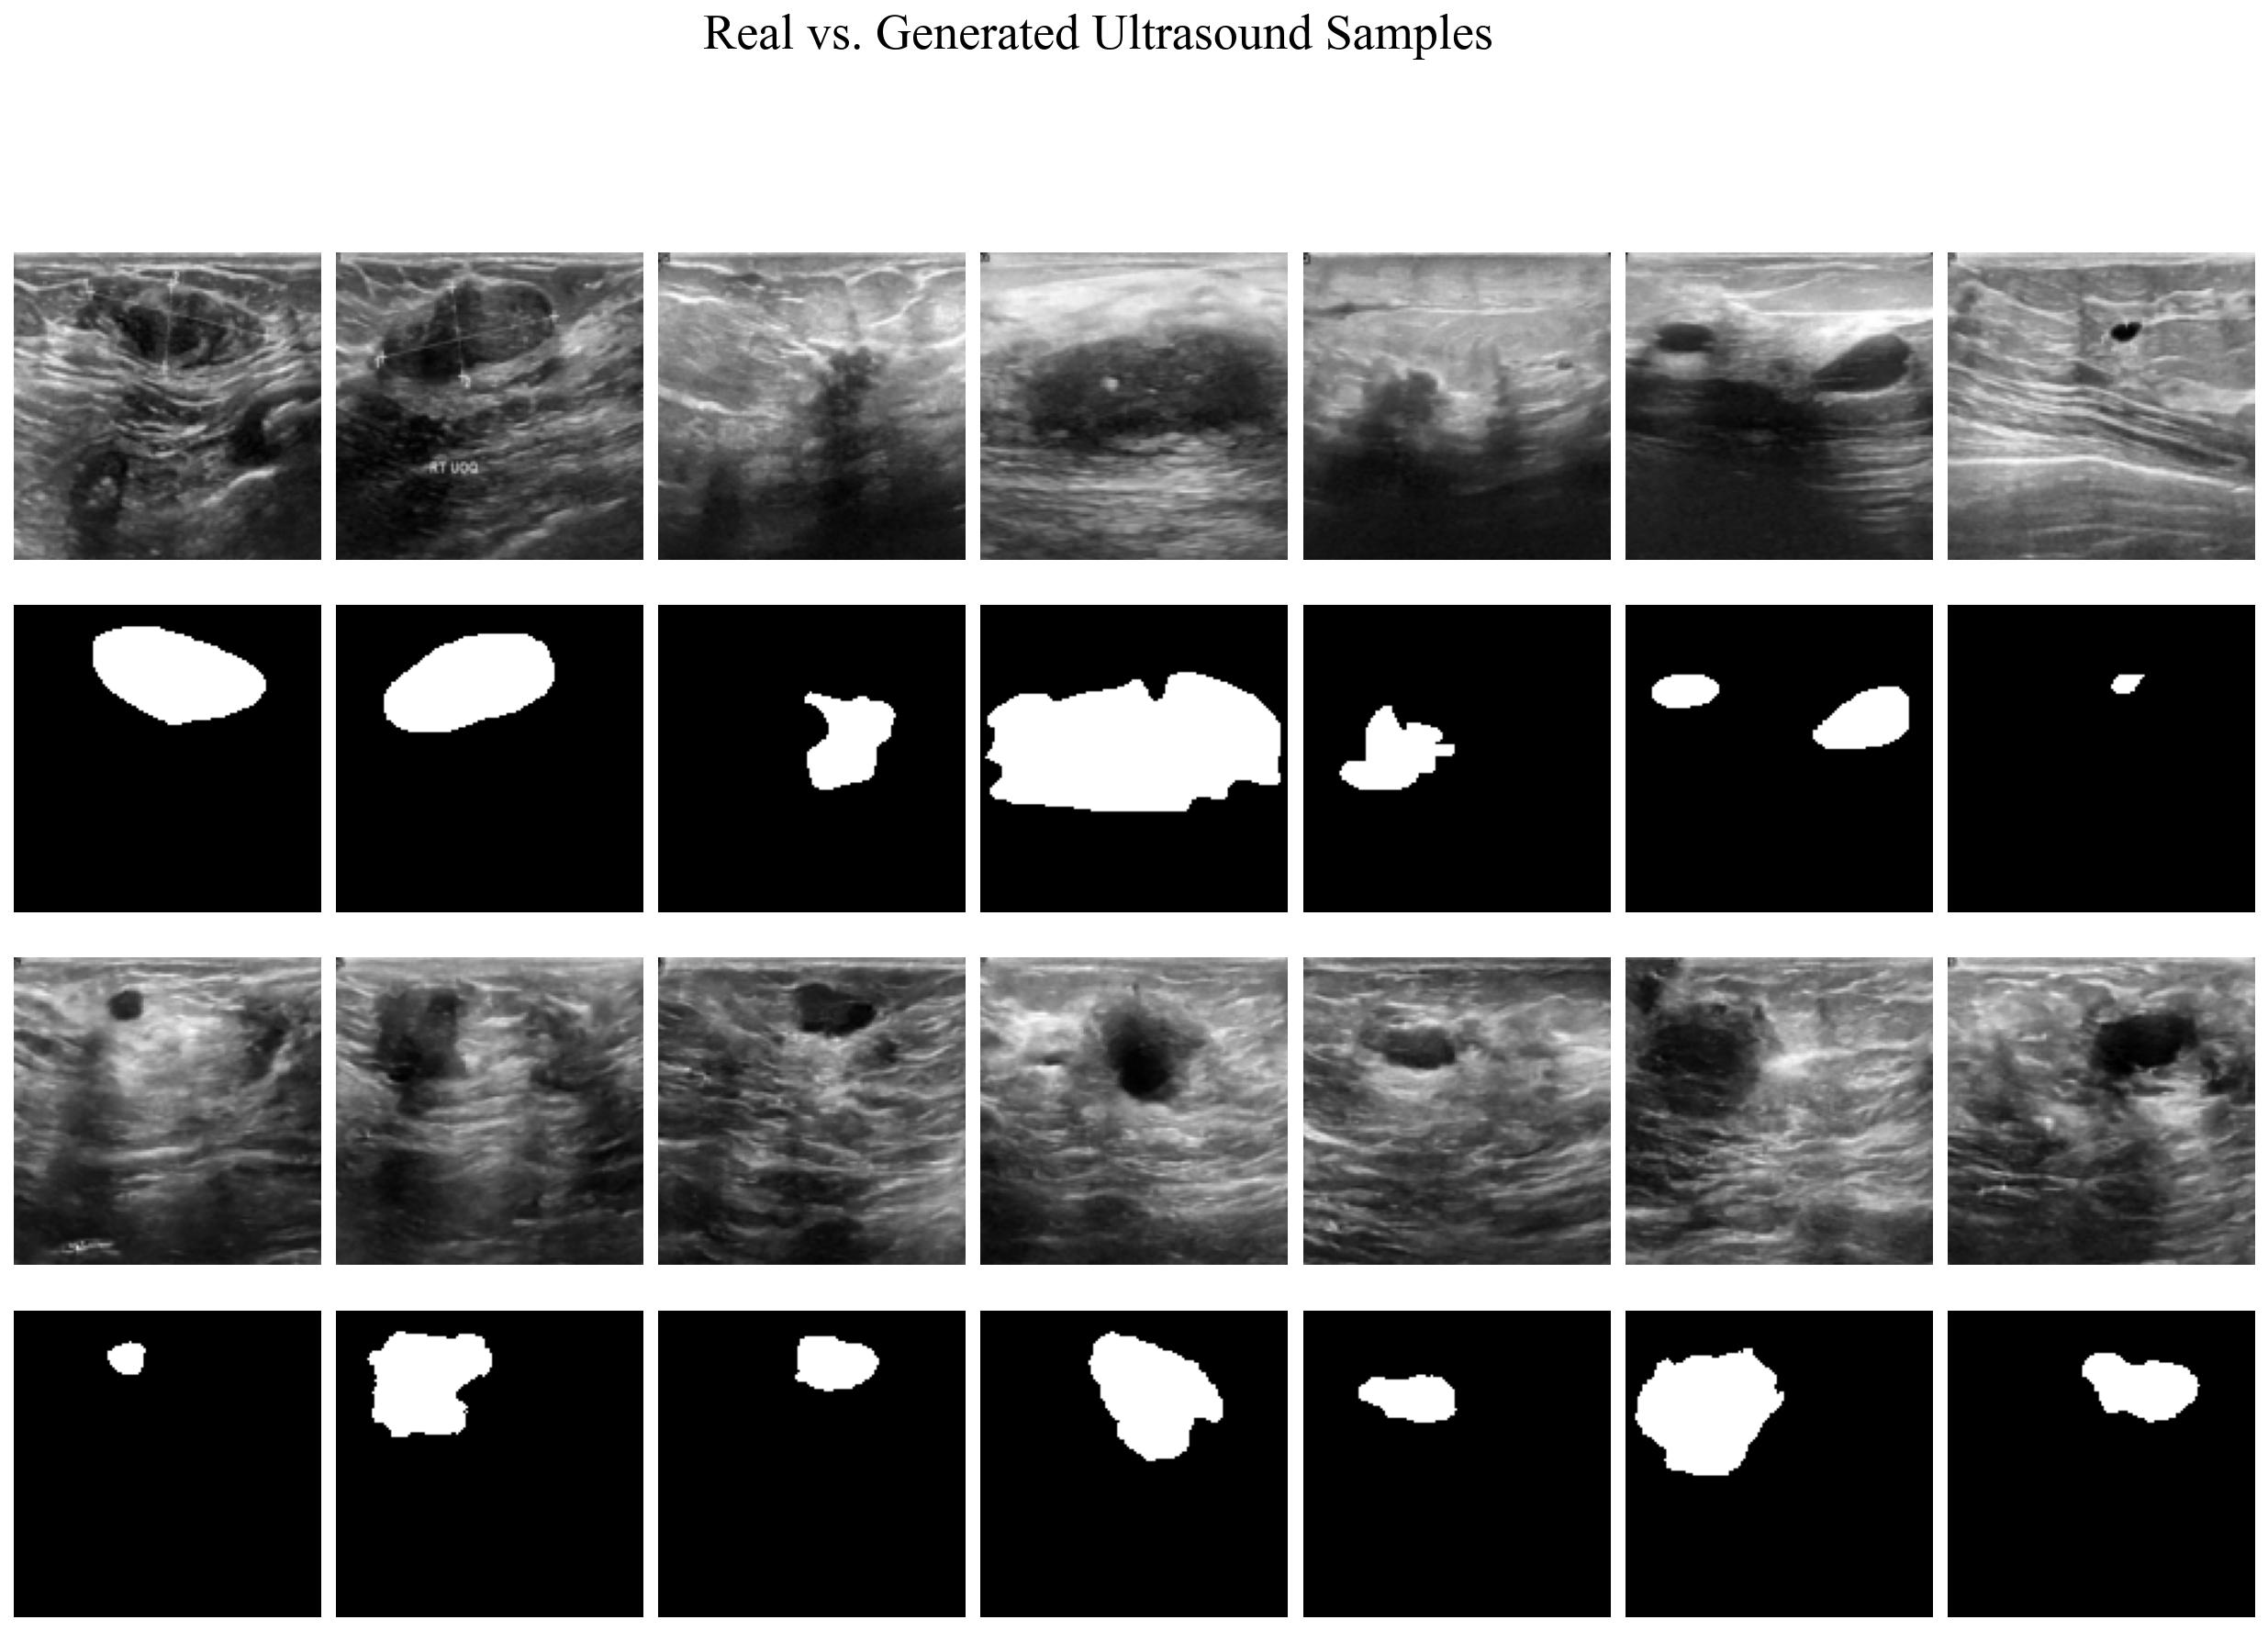
\includegraphics[width=\linewidth]{zlati_figures/real_vs_generated_v2.jpg}
    \caption{Real (rows 1--2) vs.\ generated (rows 3--4) ultrasound image--mask pairs. Generated samples exhibit realistic texture and spatially consistent masks.}
    \label{fig:real_vs_gen}
\end{figure}

\subsection{Distributional Analysis}

To assess whether synthetic samples cover the real data distribution, we perform t-SNE dimensionality reduction~\cite{van2008} on the combined set of 556 real and 1{,}000 synthetic samples (Figure~\ref{fig:tsne}). The real and synthetic samples exhibit strong overlap with no apparent clustering by source, indicating that the generative model produces diverse samples spanning the full data manifold rather than collapsing to a subset of modes.

\begin{figure}[t]
    \centering
    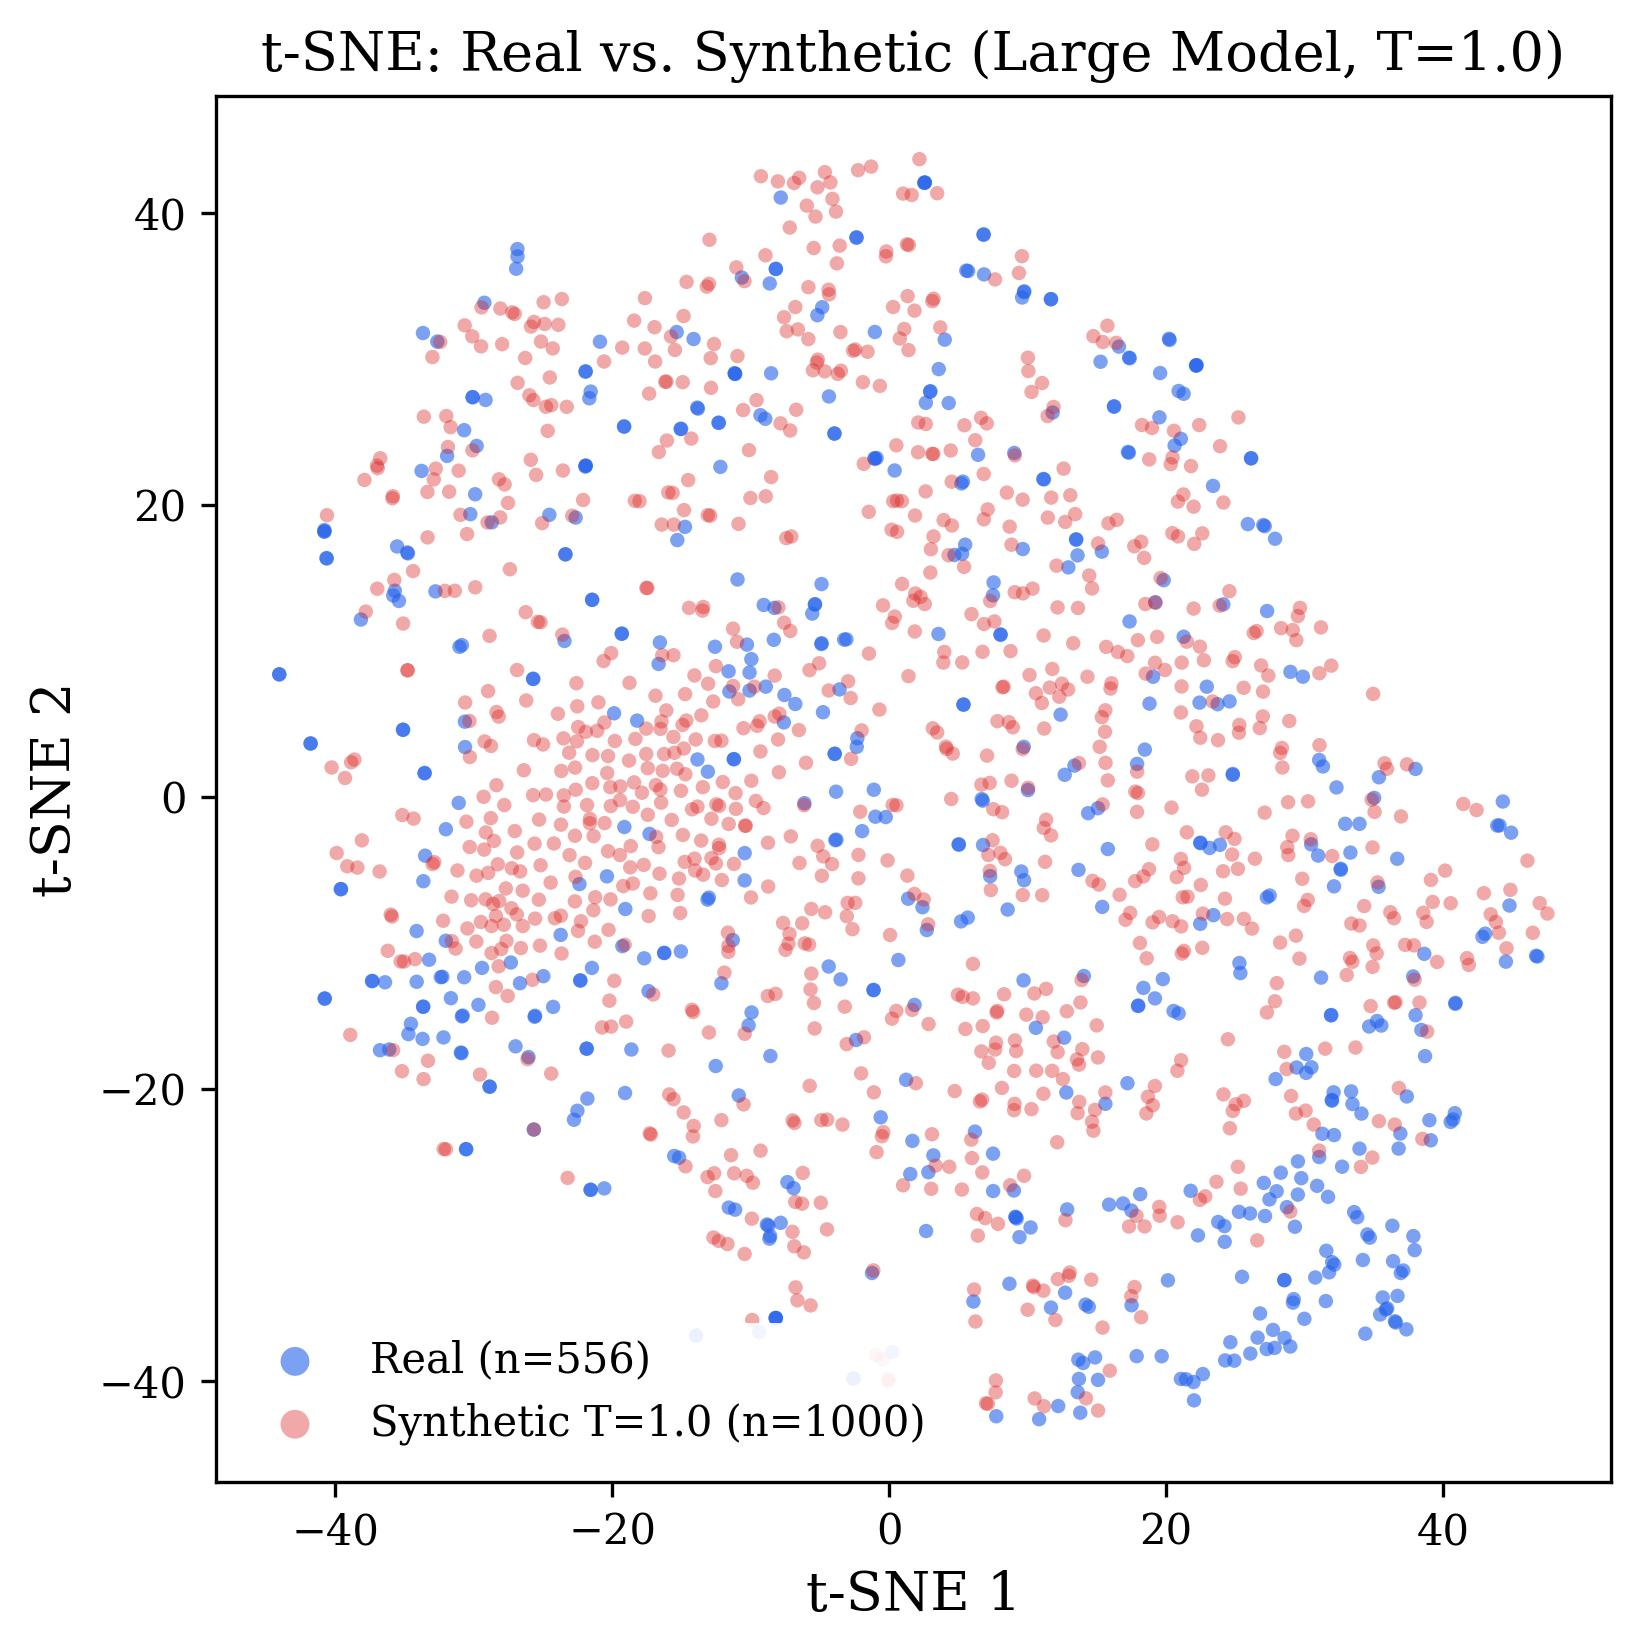
\includegraphics[width=0.9\linewidth]{zlati_figures/tsne_large_t1.0.jpg}
    \caption{t-SNE visualization of real (blue, $n=556$) and synthetic (red, $n=1{,}000$) samples, showing strong distributional overlap.}
    \label{fig:tsne}
\end{figure}

\subsection{Segmentation Performance}

Qualitative segmentation predictions from the baseline model are shown in Figure~\ref{fig:seg_qual}, demonstrating accurate lesion delineation on the held-out test set.

\begin{figure}[t]
    \centering
    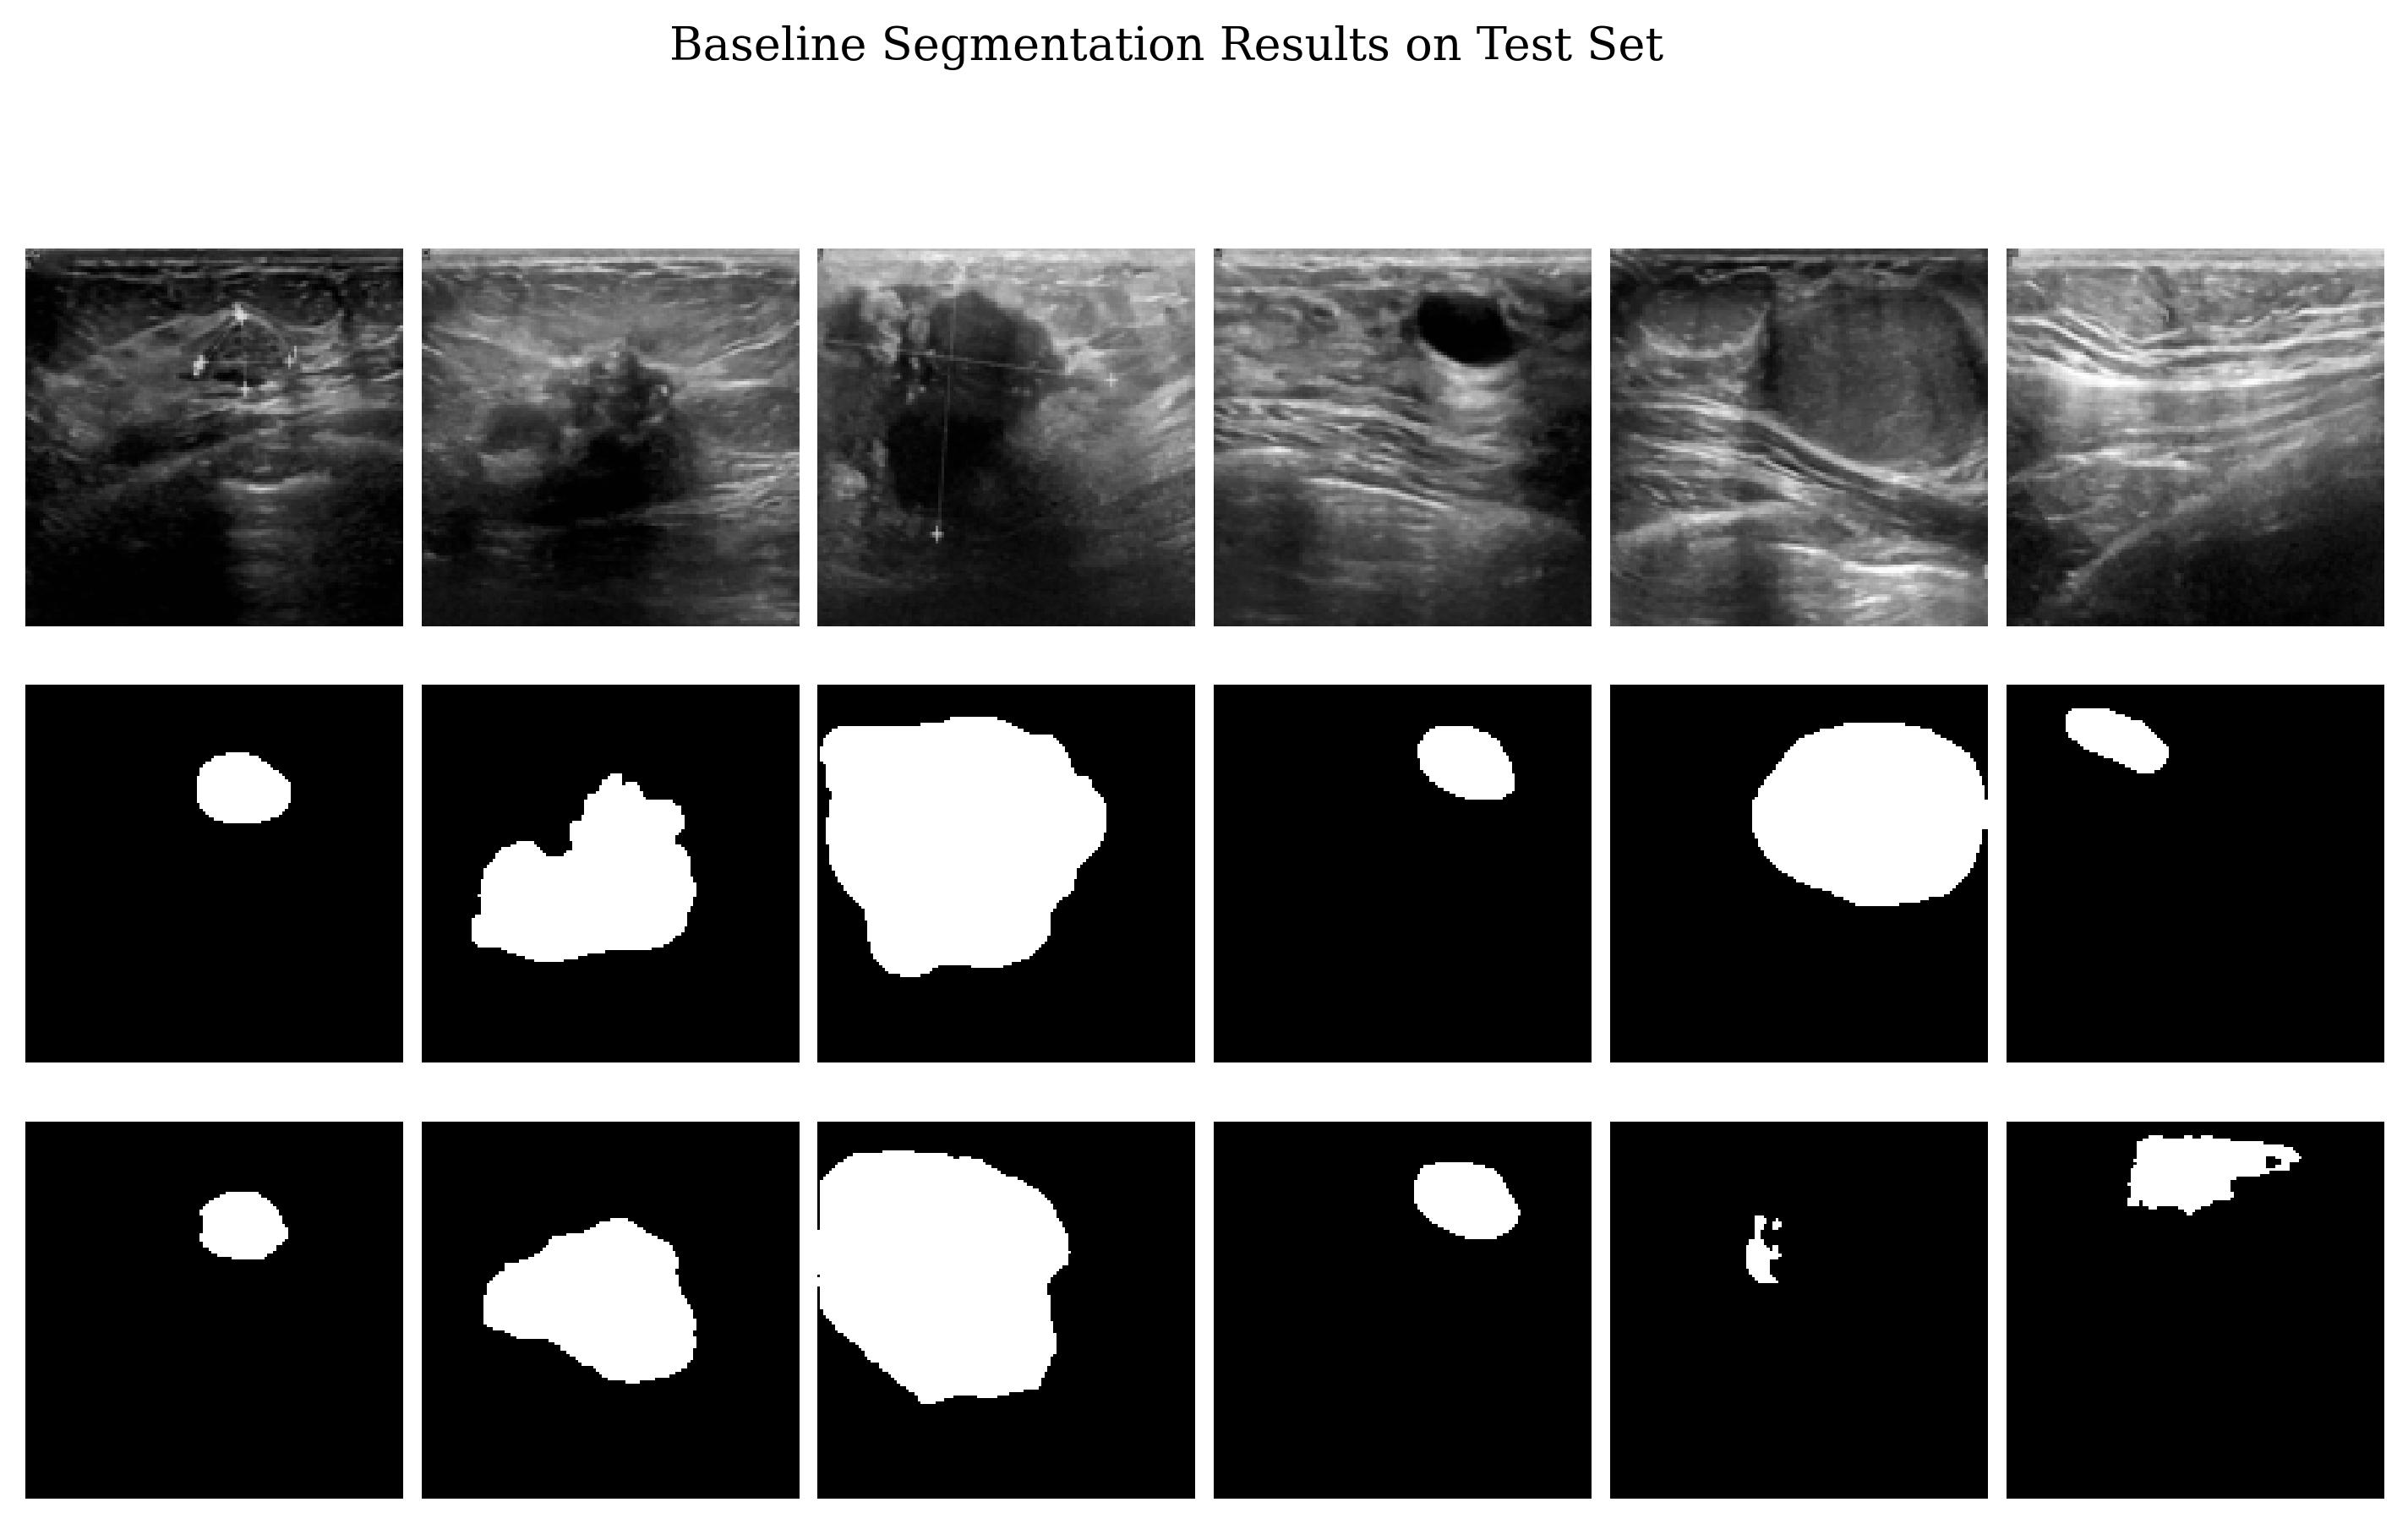
\includegraphics[width=\linewidth]{zlati_figures/seg_qualitative_baseline.jpg}
    \caption{Segmentation results on test samples. Top: input. Middle: ground truth. Bottom: prediction.}
    \label{fig:seg_qual}
\end{figure}

Table~\ref{tab:comparison} presents the key comparison between baseline and synthetic-augmented configurations. Synthetic augmentation consistently improves segmentation across all tested ratios, with the best results at 1{,}000 synthetic samples (Dice $0.823 \pm 0.004$), representing a 3.3\% improvement over the baseline (Dice $0.797 \pm 0.014$). Notably, performance improves monotonically with the exception of a dip at 400 samples, and the variance decreases substantially---the standard deviation of Dice drops from 0.014 (baseline) to 0.004 (+1{,}000), indicating that synthetic augmentation also stabilizes training.

\begin{table}[t]
    \centering
    \caption{Segmentation performance (mean $\pm$ std, 3 seeds). Best results in bold.}
    \label{tab:comparison}
    \begin{tabular}{@{}rcccc@{}}
        \toprule
        Synthetic & Dice & IoU & Precision & Recall \\
        \midrule
        0 (baseline) & $.797{\scriptstyle\pm.014}$ & $.664{\scriptstyle\pm.021}$ & $.825{\scriptstyle\pm.062}$ & $.786{\scriptstyle\pm.060}$ \\
        +300 & $.820{\scriptstyle\pm.012}$ & $.699{\scriptstyle\pm.016}$ & $.851{\scriptstyle\pm.004}$ & $.795{\scriptstyle\pm.024}$ \\
        +1{,}000 & $\mathbf{.823{\scriptstyle\pm.004}}$ & $\mathbf{.700{\scriptstyle\pm.005}}$ & $\mathbf{.853{\scriptstyle\pm.004}}$ & $\mathbf{.800{\scriptstyle\pm.004}}$ \\
        \bottomrule
    \end{tabular}
\end{table}

The full trend across all augmentation ratios is shown in Figure~\ref{fig:dice_iou}. Both Dice and IoU remain above or near the baseline across the entire range, with no degradation even at the highest ratio (1.8:1 synthetic-to-real).

\begin{figure}[t]
    \centering
    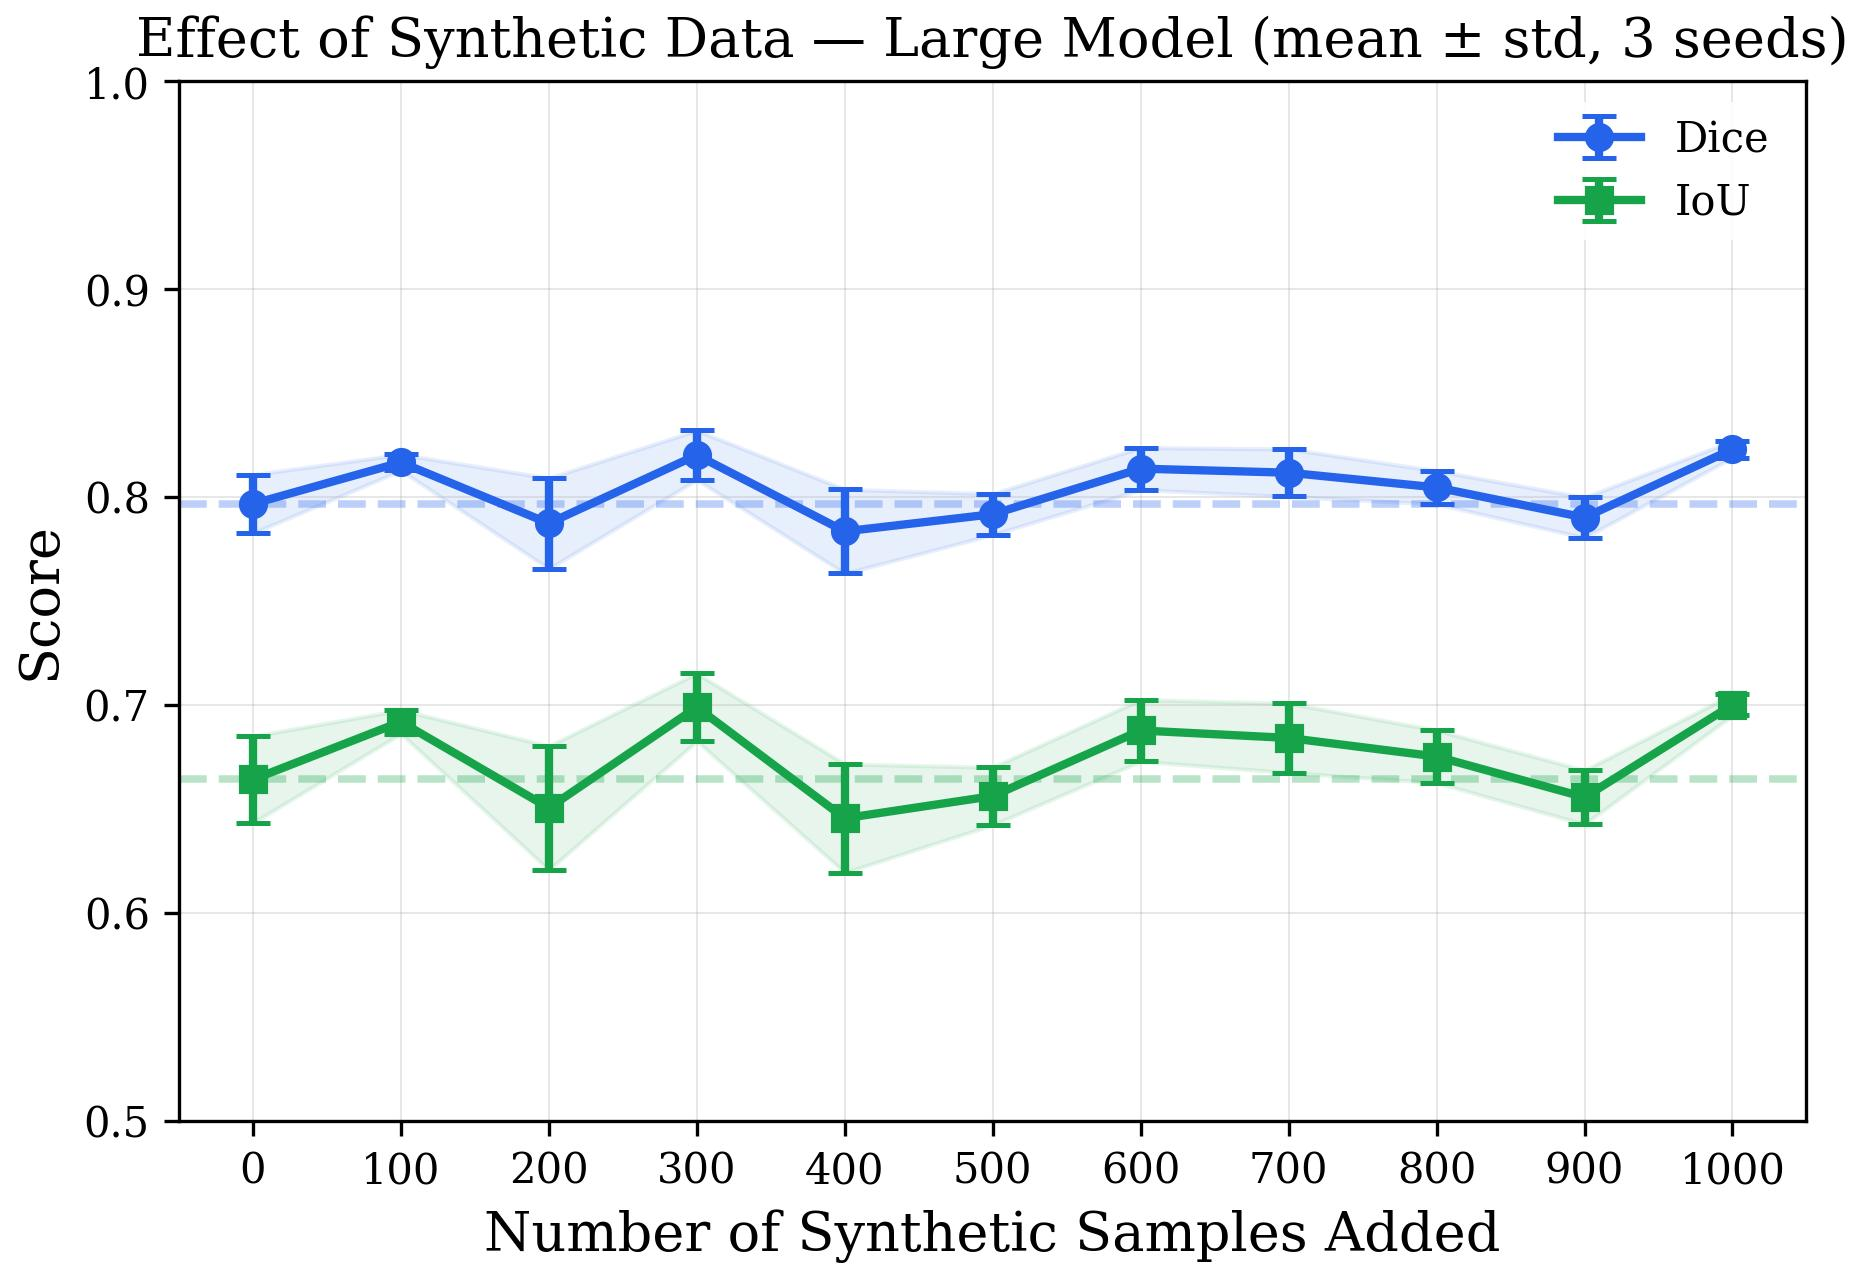
\includegraphics[width=\linewidth]{zlati_figures/experiment_dice_iou_3seeds.jpg}
    \caption{Dice and IoU vs.\ number of synthetic samples added (mean $\pm$ std, 3 seeds). Dashed lines indicate baseline performance.}
    \label{fig:dice_iou}
\end{figure}

% ============================================================
\section{Discussion}
\label{sec:discussion}

Our results suggest that synthetic data from a flow matching generative model can improve downstream segmentation, though the gains are moderate and should be interpreted in context.

\textbf{Synthetic augmentation improves performance.} The best configuration (+1{,}000 synthetic) achieves a Dice of $0.823 \pm 0.004$ compared to $0.797 \pm 0.014$ for the baseline. While the absolute improvement is modest, the gains are consistent across metrics and achieved without additional real data collection or annotation cost. Notably, synthetic augmentation also reduces training variance: the Dice standard deviation drops from 0.014 to 0.004, suggesting a regularizing effect that stabilizes training across random initializations.

\textbf{Generative model capacity matters.} In preliminary experiments with a smaller 26.6M-parameter model, synthetic augmentation showed diminishing returns beyond 300 samples. Scaling to 106.4M parameters improved sample quality sufficiently that augmentation remained beneficial across all tested ratios, underscoring that the quality of the generative model is a key factor in determining the utility of synthetic data.

\textbf{Joint image--mask generation.} By concatenating images and masks as two-channel inputs, the generative model learns their joint distribution, ensuring spatial consistency between generated images and their corresponding masks---a property that would not be guaranteed by generating them independently.

\textbf{Limitations.} The dataset comprises only 647 images at $128 \times 128$ resolution, which limits both the generative model's capacity and the statistical power of downstream experiments. The test set contains only 46 images, and results are averaged over three seeds; larger-scale validation is needed to confirm these findings. We do not compute the Fr\'{e}chet Inception Distance (FID)~\cite{heusel2017} as its reliance on Inception features pretrained on natural images makes it poorly suited for evaluating domain-specific medical image quality. Future work should explore domain-specific perceptual metrics, higher resolutions, and conditional generation.

% ============================================================
\section{Related Work}
\label{sec:related}

Synthetic data for medical imaging has been explored across modalities. GANs have been applied to retinal fundus images~\cite{costa2018}, chest X-rays~\cite{jang2023}, and histopathology~\cite{hou2019}. Diffusion models have more recently been applied to medical image synthesis, including brain MRI~\cite{pinaya2022} and chest CT~\cite{khader2023}. The effect of synthetic augmentation on segmentation performance has been studied in cardiac MRI~\cite{zhang2022}, where GAN-generated images improved segmentation accuracy.

Flow matching, introduced by Lipman et al.~\cite{lipman2023} and concurrently by Liu et al.~\cite{liu2023}, has gained attention for its training simplicity and sample quality. Ozbey et al.~\cite{ozbey2025} recently applied optimal transport flow matching to medical image synthesis on echocardiography and brain MRI, using mask-conditional generation and evaluating quality via FID. However, their work does not investigate the downstream effect of synthetic augmentation on segmentation performance, nor does it study the optimal ratio of synthetic-to-real data. Moreover, FID---which relies on Inception features pretrained on natural images---is of limited utility in data-scarce medical imaging domains where the target distribution differs substantially from ImageNet. Our work focuses directly on the downstream question: does synthetic data improve segmentation on unseen real data, and if so, how much is needed?

Additionally, while latent diffusion approaches~\cite{pinaya2022} offer scalability via a pretrained VAE, they introduce a dependency on a domain-appropriate encoder and risk reconstruction artifacts. Our pixel-space approach avoids this entirely, operating directly on image pixels to preserve fine-grained spatial detail.

% ============================================================
\section{Conclusion}
\label{sec:conclusion}

We have presented a pipeline for generating synthetic breast ultrasound image--mask pairs using UNet-based flow matching, and demonstrated its utility for augmenting segmentation model training. Our systematic experiments show that synthetic augmentation from a 106.4M-parameter generative model consistently improves segmentation performance on unseen data, with the best configuration yielding a 3.3\% Dice improvement and substantially reduced training variance. Distributional analysis confirms that generated samples faithfully span the real data manifold. These findings support the integration of flow matching generative models into medical imaging workflows, offering a scalable, privacy-preserving approach to addressing annotated data scarcity.

% ============================================================
\bibliographystyle{unsrt}
\begin{thebibliography}{99}

\bibitem{litjens2017}
G.~Litjens et al., ``A survey on deep learning in medical image analysis,'' \textit{Medical Image Analysis}, vol.~42, pp.~60--88, 2017.

\bibitem{willemink2020}
M.~J.~Willemink et al., ``Preparing medical imaging data for machine learning,'' \textit{Radiology}, vol.~295, no.~1, pp.~4--15, 2020.

\bibitem{johnson2019}
J.~M.~Johnson and T.~M.~Khoshgoftaar, ``Survey on deep learning with class imbalance,'' \textit{Journal of Big Data}, vol.~6, no.~1, pp.~1--54, 2019.

\bibitem{goodfellow2014}
I.~Goodfellow et al., ``Generative adversarial nets,'' in \textit{Advances in Neural Information Processing Systems}, 2014.

\bibitem{kingma2014}
D.~P.~Kingma and M.~Welling, ``Auto-encoding variational Bayes,'' in \textit{International Conference on Learning Representations}, 2014.

\bibitem{ho2020}
J.~Ho, A.~Jain, and P.~Abbeel, ``Denoising diffusion probabilistic models,'' in \textit{Advances in Neural Information Processing Systems}, 2020.

\bibitem{dhariwal2021}
P.~Dhariwal and A.~Nichol, ``Diffusion models beat GANs on image synthesis,'' in \textit{Advances in Neural Information Processing Systems}, 2021.

\bibitem{lipman2023}
Y.~Lipman, R.~T.~Q.~Chen, H.~Ben-Hamu, M.~Nickel, and M.~Le, ``Flow matching for generative modeling,'' in \textit{International Conference on Learning Representations}, 2023.

\bibitem{liu2023}
X.~Liu, C.~Gong, and Q.~Liu, ``Flow straight and fast: Learning to generate and transfer data with rectified flow,'' in \textit{International Conference on Learning Representations}, 2023.

\bibitem{sohl2015}
J.~Sohl-Dickstein, E.~Weiss, N.~Maheswaranathan, and S.~Ganguli, ``Deep unsupervised learning using nonequilibrium thermodynamics,'' in \textit{International Conference on Machine Learning}, 2015.

\bibitem{ronneberger2015}
O.~Ronneberger, P.~Fischer, and T.~Brox, ``U-Net: Convolutional networks for biomedical image segmentation,'' in \textit{MICCAI}, 2015.

\bibitem{peebles2023}
W.~Peebles and S.~Xie, ``Scalable diffusion models with transformers,'' in \textit{International Conference on Computer Vision}, 2023.

\bibitem{von-platen2022}
P.~von Platen et al., ``Diffusers: State-of-the-art diffusion models,'' \url{https://github.com/huggingface/diffusers}, 2022.

\bibitem{van2008}
L.~van der Maaten and G.~Hinton, ``Visualizing data using t-SNE,'' \textit{Journal of Machine Learning Research}, vol.~9, pp.~2579--2605, 2008.

\bibitem{al-dhabyani2020}
W.~Al-Dhabyani, M.~Gomaa, H.~Khaled, and A.~Fahmy, ``Dataset of breast ultrasound images,'' \textit{Data in Brief}, vol.~28, p.~104863, 2020.

\bibitem{heusel2017}
M.~Heusel, H.~Ramsauer, T.~Unterthiner, B.~Nessler, and S.~Hochreiter, ``GANs trained by a two time-scale update rule converge to a local Nash equilibrium,'' in \textit{Advances in Neural Information Processing Systems}, 2017.

\bibitem{chen2022}
R.~J.~Chen et al., ``Synthetic data in machine learning for medicine and healthcare,'' \textit{Nature Biomedical Engineering}, vol.~5, pp.~493--497, 2021.

\bibitem{costa2018}
P.~Costa et al., ``End-to-end adversarial retinal image synthesis,'' \textit{IEEE Transactions on Medical Imaging}, vol.~37, no.~3, pp.~781--791, 2018.

\bibitem{jang2023}
R.~Jang et al., ``Assessment of the robustness of a deep learning model for the generation of synthetic chest X-ray images,'' \textit{Radiology: Artificial Intelligence}, vol.~5, no.~3, 2023.

\bibitem{hou2019}
L.~Hou et al., ``Robust histopathology image analysis: To label or to synthesize?,'' in \textit{CVPR}, 2019.

\bibitem{pinaya2022}
W.~H.~L.~Pinaya et al., ``Brain imaging generation with latent diffusion models,'' in \textit{MICCAI Workshop on Deep Generative Models}, 2022.

\bibitem{khader2023}
F.~Khader et al., ``Denoising diffusion probabilistic models for 3D medical image generation,'' \textit{Scientific Reports}, vol.~13, 2023.

\bibitem{zhang2022}
L.~Zhang et al., ``Generative adversarial networks for cardiac MRI segmentation augmentation,'' in \textit{Statistical Atlases and Computational Models of the Heart}, 2022.

\bibitem{ozbey2025}
M.~Ozbey et al., ``Flow matching for medical image synthesis: Bridging the gap between speed and quality,'' \textit{arXiv preprint arXiv:2503.00266}, 2025.

\end{thebibliography}

\end{document}
